\documentclass[tikz]{standalone}
\usepackage{tikz}
\begin{document}
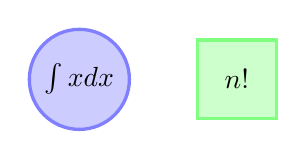
\begin{tikzpicture}
[L1Node/.style={circle,   draw=blue!50, fill=blue!20, very thick, minimum size=10mm},
L2Node/.style={rectangle,draw=green!50,fill=green!20,very thick, minimum size=10mm}]
\node[L1Node] (n1) at (0, 0){$\int x dx$};
\node[L2Node] (n2) at (2, 0){$n!$};
\end{tikzpicture}
\end{document}
